\documentclass[usepdftitlre=false, debug]{beamer}

\usepackage[francais]{babel}
\usepackage[T1]{fontenc}
\usepackage[ansinew]{inputenc}
\usepackage{lmodern}
\usepackage{graphicx}
\usepackage{listings}
\usepackage{color}
\usepackage{pgf}
\usepackage{tikz}
\usetikzlibrary{arrows,automata}



%%%%%%%%%%%%%%%%%%%%%%%%%%%%%%%%%%%%%%%%%%%%%%%%%%%%%%%%%%%%%%%%%%%%%%%%%%%%%%%%%%%%%%%%%%%%%%%%
\usetheme{Rochester}
\usecolortheme{default}

\title{Cryptographie}
\author{Mathis Deloge, Antoine Petot, Ange Picard}
%\institute{IUT Informatique Dijon / Auxerre}
\date{Dimanche 4 d�cembre 2016}
%%%%%%%%%%%%%%%%%%%%%%%%%%%%%%%%%%%%%%%%%%%%%%%%%%%%%%%%%%%%%%%%%%%%%%%%%%%%%%%%%%%%%%%%%%%%%%%%



\definecolor{mygreen}{rgb}{0,0.6,0}
\definecolor{mygray}{rgb}{0.5,0.5,0.5}
\definecolor{mymauve}{rgb}{1,0,0}

\lstset{ %
  backgroundcolor=\color{gray!30!white},   % choose the background color
  basicstyle=\small\ttfamily,        % size of fonts used for the code
  breaklines=true,                 % automatic line breaking only at whitespace
  captionpos=b,                    % sets the caption-position to bottom
  commentstyle=\color{mygreen},    % comment style
  escapeinside={\%*}{*)},          % if you want to add LaTeX within your code
  keywordstyle=\color{blue},       % keyword style
  stringstyle=\color{mymauve},     % string literal style
	numbers=left,
	frame=leftline,
	xleftmargin=42pt
}

\setbeamertemplate{navigation symbols}{%
\insertbackfindforwardnavigationsymbol
}

\setbeamercolor{background canvas}{bg=yellow!10!white}

\AtBeginSection[]
{
  \begin{frame}
  \frametitle{Sommaire}
  \tableofcontents[currentsection, hideothersubsections]
  \end{frame}
}

\begin{document}

\begin{frame}
	\titlepage
\end{frame}

\section{Pr�sentation du sujet}
\subsection{Le sujet}
\begin{frame}
	\frametitle{Le sujet}
	\pause
	\begin{block}{Descriptif}
	Impl�mentation de deux programmes permettant le codage et le d�codage d'information num�riques suivant les deux principes suivant :
	\begin{itemize}
	 \item Echange de cl� de Diffie-Hellman
	 \item Chiffrement par transposition
	\end{itemize}
	\end{block}
\end{frame}

\subsubsection{Diffie-Hellamn}
\begin{frame}
	\frametitle{Diffie-Hellman}
	\begin{block}{Principe}
	\begin{itemize}
	 \item Alice et Bob choisissent un groupe fini G d'ordre n et un g�n�rateur g de ce groupe publiquement
	 \item Alice choisi au hasard a tel que 1 < a < n puis communique � Bob ga
	 \item Bob choisi au hasard b tel que 1 < b < n puis communique � Alice gb
	 \item Alice �l�ve � la puissance a le nombre communiqu� par Bob
	 \item Bob �l�ve � la puissance b le nombre communiqu� par Alice
	 \item Alice et Bob connaissent le nombre g(ab) impssible � d�terminer par Eve
	\end{itemize}
	\end{block}
\end{frame}
\begin{frame}
	\frametitle{Diffie-Hellman}
	\begin{center}
	 	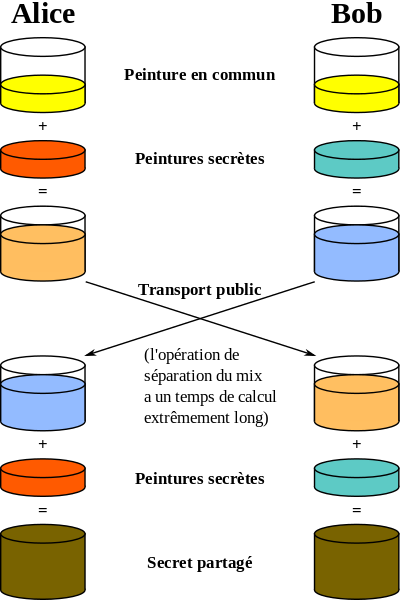
\includegraphics[width=5cm]{Images/Diffie-Hellman.png}
	\end{center}
\end{frame}

\subsubsection{Chiffrement par transposition}
\begin{frame}
	\frametitle{Chiffrement par transposition}
	\begin{block}{Principe}
	\begin{itemize}
	 \item Avec le chiffrement par transposition, il est n�cessaire que Alice et Bob connaissent une cl� de chiffrement.
	 \item  Lors du chiffrement par transposition, on d�coupe le texte cod� en bloc de la taille de la cl� de chiffrement pour ensuite permuter l'ordre des caract�re � l'int�rieur de ces blocs en suivant le cl� de chiffrement.
	 \item Pour d�chiffrer un message, il suffit de remettre les caract�res � leur place au sein de chaque bloc de texte en s'aidant de la cl� de chiffrement
	\end{itemize}
	\end{block}	
\end{frame}

\begin{frame}
	\frametitle{Chiffrement par transposition}
	 On peut repr�senter la chiffrement d'un message par transposition � l'aide d'un tableau :
	 \begin{center}
	 	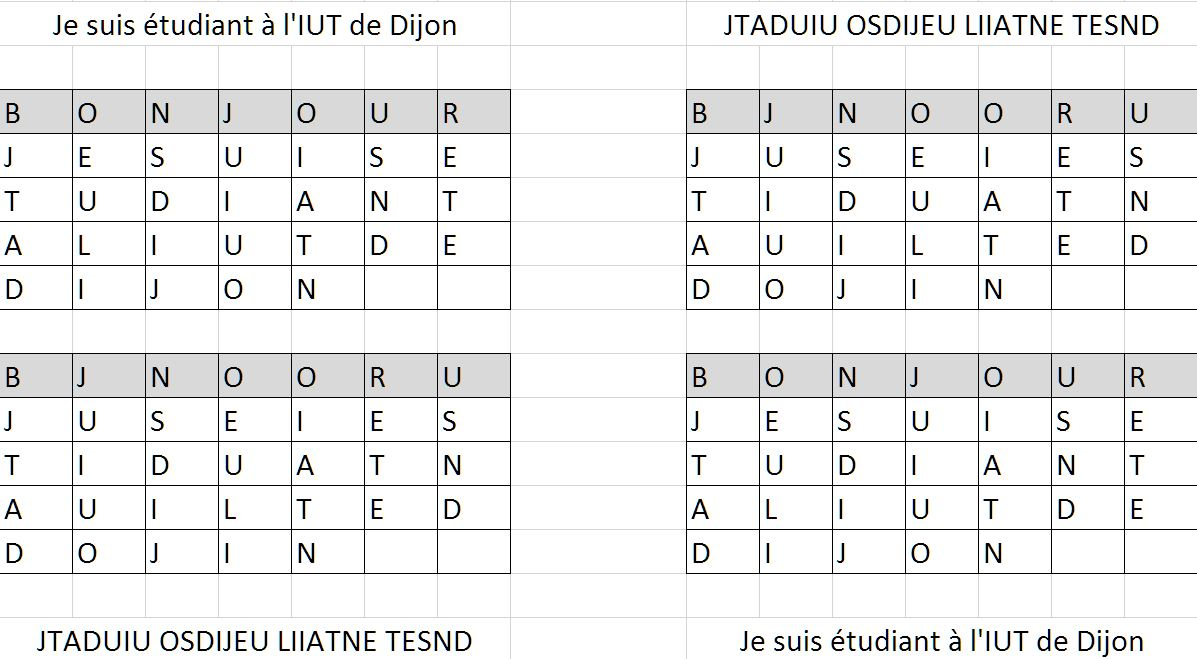
\includegraphics[width=9cm]{Images/tableau.jpg}
	\end{center}
\end{frame}

\subsection{Prolongements possibles}
\begin{frame}
	\frametitle{Prolongements possibles}
	\begin{block}{Les diff�rents prolongements du sujet}
	 \begin{itemize}
	  \item Conseillez Alice et Bob sur le choix du protocole de partage de cl�.
	  \item Si Alice et Bob ne s'�taient pas connus � l'universit�, auraient-ils pu utiliser la m�thode propos�e par Bob ? Et celle propos�e par Alice ?
	  \item Attaque de l'homme du milieu avec Diffie-Hellman.
	  \item Algorithme ``baby step giant step'' et r�solution du probl�me du logarithme discret dans Diffie-Hellman.
	  \item Protocole d'attaque pour le chiffrement par transposition.
	 \end{itemize}
	\end{block}

\end{frame}










\section{Pr�sentation des programme}
\subsection{Diffie-Hellman}
\begin{frame}
	\frametitle{Diffie-Hellman} 
	\pause

\end{frame}
\subsection{Chiffrement par transposition}
\begin{frame}
	\frametitle{Chiffrement par transposition} 
	\pause

\end{frame}


\section{R�sultats}
\begin{frame}
	\frametitle{R�sultats}
	\pause

\end{frame}


\section{Conclusion}
\begin{frame}
 \frametitle{Conclusion}
 \pause


\end{frame}


\begin{frame}
  \frametitle{Sommaire}
  \tableofcontents
\end{frame}

\end{document}